% Demonstrating Improved Accuracy

\frame{ \frametitle{Demonstrating Improved Accuracy}
  We have an approximation!!
  \pause

  But is it more accurate? ...
  \pause
  Answer: Yes!
}

%% Visual Inspection
\frame{ \frametitle{Demonstrating Improved Accuracy: Visual}
  The easiest way of gauging accuracy is by visual inspection.
}
\frame{ \frametitle{Demonstrating Improved Accuracy: Visual}
  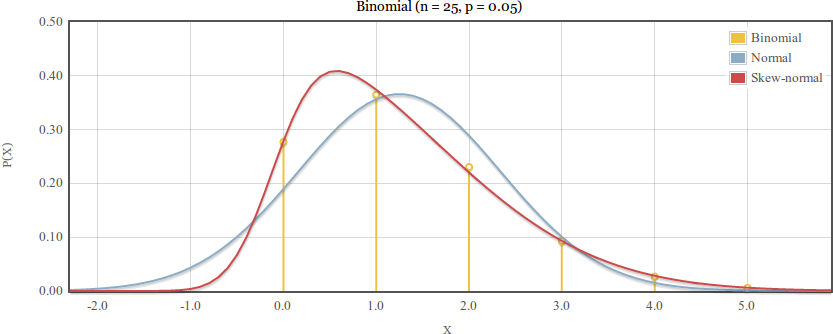
\includegraphics[width=\textwidth]{../images/comparison-n25-p005.png}
}
\frame{ \frametitle{Demonstrating Improved Accuracy: Visual}
  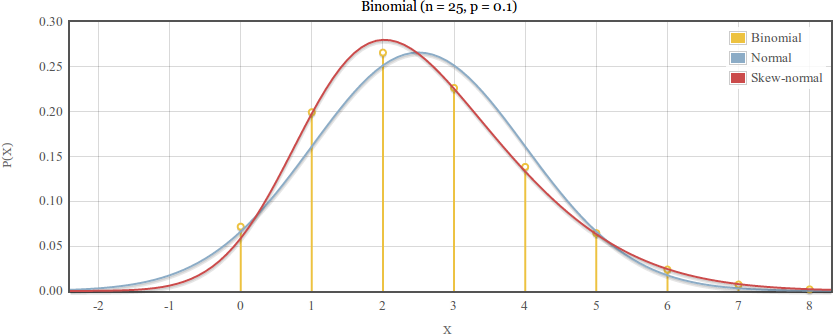
\includegraphics[width=\textwidth]{../images/comparison-n25-p01.png}
}
\frame{ \frametitle{Demonstrating Improved Accuracy: Visual}
  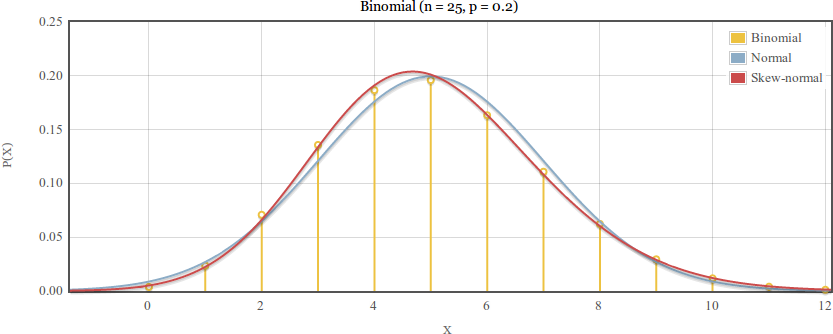
\includegraphics[width=\textwidth]{../images/comparison-n25-p02.png}
}
\frame{ \frametitle{Demonstrating Improved Accuracy: Visual}
  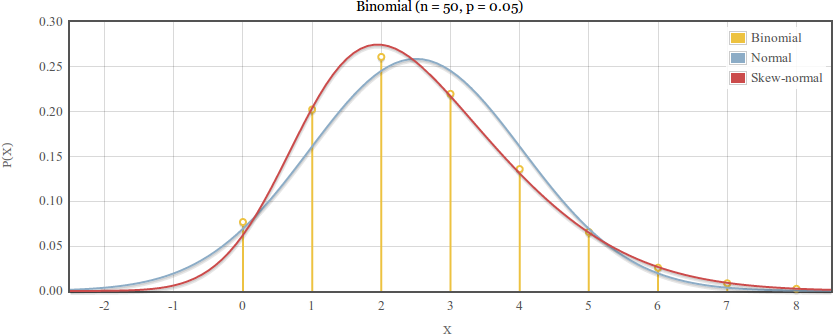
\includegraphics[width=\textwidth]{../images/comparison-n50-p005.png}
}
\frame{ \frametitle{Demonstrating Improved Accuracy: Visual}
  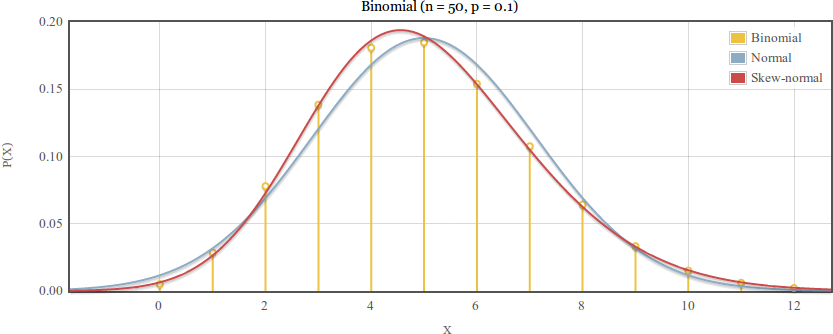
\includegraphics[width=\textwidth]{../images/comparison-n50-p01.png}
}
\frame{ \frametitle{Demonstrating Improved Accuracy: Visual}
  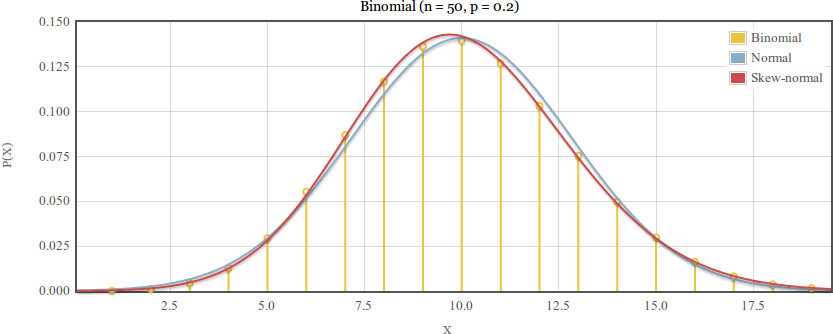
\includegraphics[width=\textwidth]{../images/comparison-n50-p02.png}
}
\frame{ \frametitle{Demonstrating Improved Accuracy: Visual}
  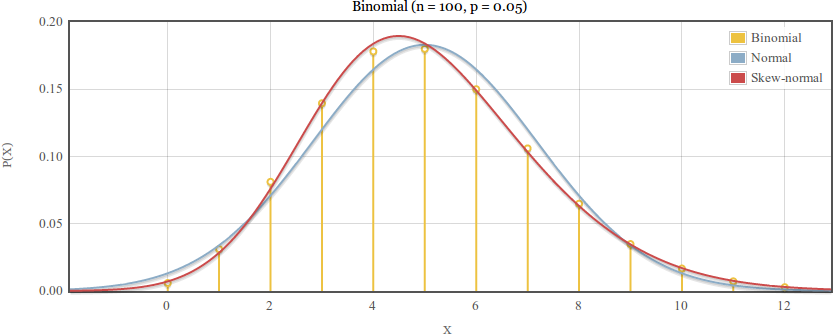
\includegraphics[width=\textwidth]{../images/comparison-n100-p005.png}
}
\frame{ \frametitle{Demonstrating Improved Accuracy: Visual}
  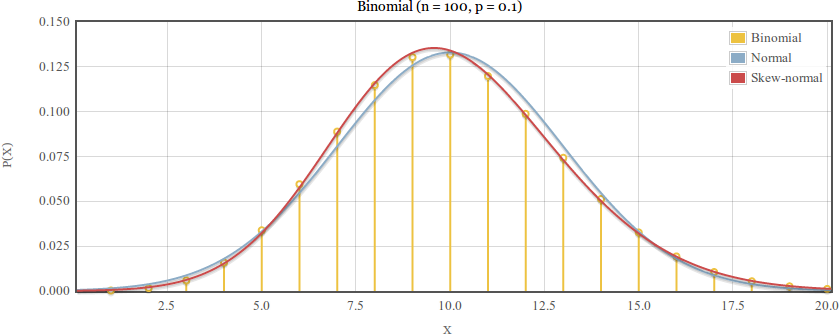
\includegraphics[width=\textwidth]{../images/comparison-n100-p01.png}
}
\frame{ \frametitle{Demonstrating Improved Accuracy: Visual}
  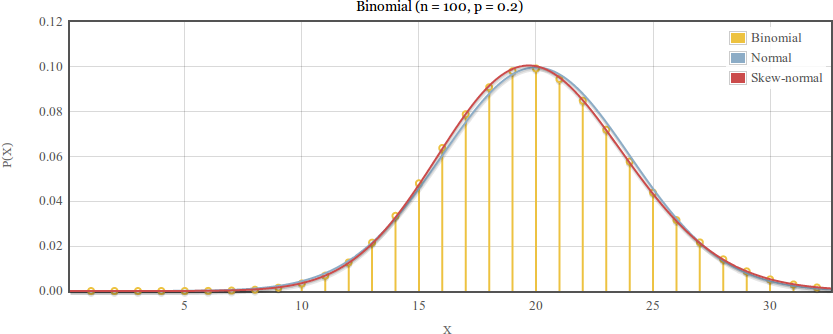
\includegraphics[width=\textwidth]{../images/comparison-n100-p02.png}
}

%% MABS
\frame{ \frametitle{Demonstrating Improved Accuracy: MABS}
  A more numerical way of gauging accuracy is the $MABS$, defined by \citet{mabs} as
  \begin{equation*}
    \textnormal{MABS}(n, p) \eq \max_{k \in \{0, 1,...,n\}} \left| F_{B(n,p)} (k) -  F_{\textnormal{appr}(n,p)}(k + 0.5) \right|.
  \end{equation*}
  \pause

  \vspace{1cm}
  (In English: The biggest vertical distance between the binomial cdf and the approximation curve.)
}
\frame{ \frametitle{Demonstrating Improved Accuracy: MABS}
  MABS as a function of $p$, with fixed $n=25$:

  \begin{center}
    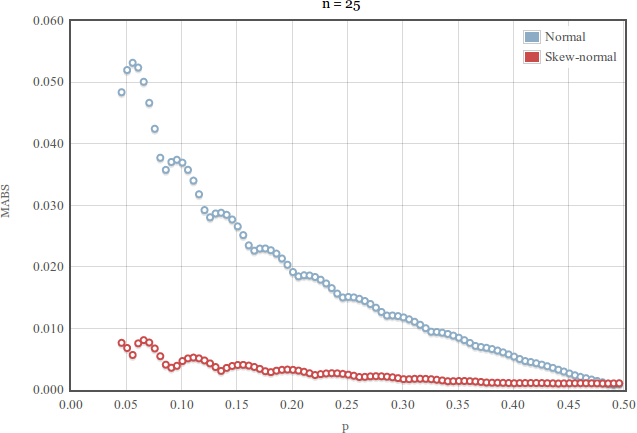
\includegraphics[width=0.8\textwidth]{../images/mabs-fixed-n25.png}
  \end{center}
}
\frame{ \frametitle{Demonstrating Improved Accuracy: MABS}
  MABS as a function of $p$, with fixed $n=100$:

  \begin{center}
    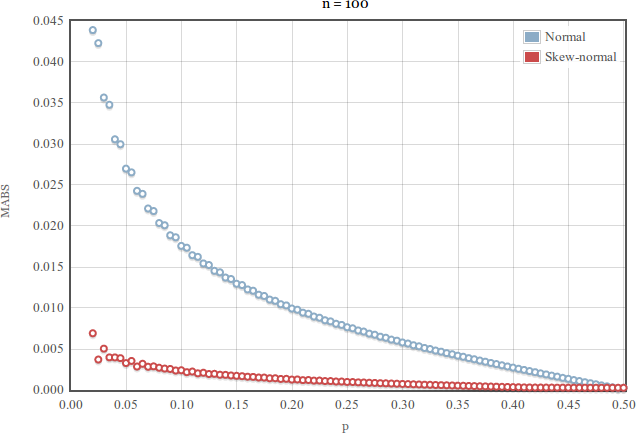
\includegraphics[width=0.8\textwidth]{../images/mabs-fixed-n100.png}
  \end{center}
}
\frame{ \frametitle{Demonstrating Improved Accuracy: MABS}
  MABS as a function of $n$, with fixed $p=0.05$:

  \begin{center}
    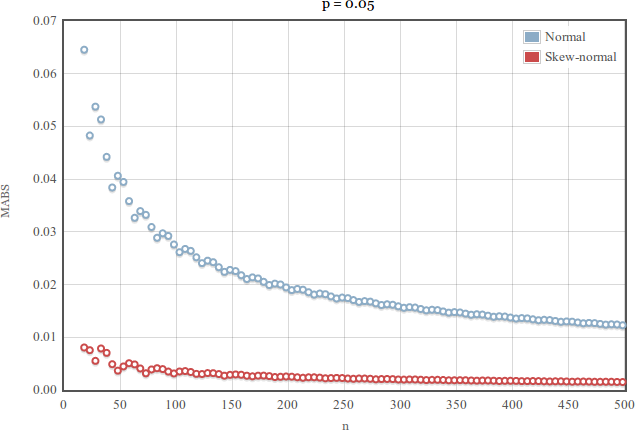
\includegraphics[width=0.8\textwidth]{../images/mabs-fixed-p005.png}
  \end{center}
}
\frame{ \frametitle{Demonstrating Improved Accuracy: MABS}
  MABS as a function of $n$, with fixed $p=0.1$:

  \begin{center}
    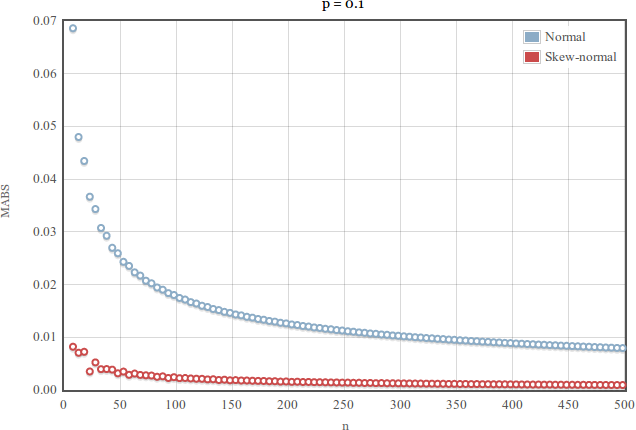
\includegraphics[width=0.8\textwidth]{../images/mabs-fixed-p01.png}
  \end{center}
}
